

\section{Underwater communication}
\label{sec:Underwatercommunication}

%\subsection{Introduction}



\subsection{Electronic part (Albin Barklund)}
\subsubsection{Description}
The light communication module is a wireless data link for short distance underwater communication between autonomous underwater vehicles (AUVs). It consists of a receiver and transmitter which utilizes power LEDs and photoresistors to send and receive data.\\\\
Bear in mind that no actual solution have been implemented and this document only summaries a couple of experiments which where conducted to prove or disprove the hypothesis in section \ref{sec:hypothesis}.
\subsubsection{Requirements}
\label{sec:req}
\begin{tabular}{l l}
Range: & 2 - 3m\\
Data rate: & 1 kbit/s\\
Input data signal: & 5V\\
Medium: & water\\
\end{tabular}\\


\begin{figure}[h]
\centering
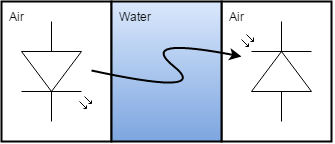
\includegraphics[width=0.5\textwidth]{medium}
\caption{Signal transistion through mediums}
\label{fig:con}
\end{figure}


\subsubsection{Hypothesis}
\label{sec:hypothesis}
With the use of power LEDs and photodiodes it is possible to create a wireless data link for underwater communication that modulates bits simply letting an asynchronous data signal control a LED which fulfill the requirements in section \ref{sec:req}


\subsubsection{Design and interface}
\textbf{Transmitter}\\
The transmitter takes an asynchronous data signal as input. The driver stage then inverts and amplifies the signal which then drives the LED. If the signal is high then the LED is turned off and if the signal is low then the LED is turned on.

\begin{figure}[h]
\centering
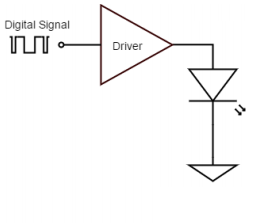
\includegraphics[width=0.4\textwidth]{trans}
\caption{The transmitter}
\label{fig:trans}
\end{figure}

 
 \textbf{Receiver}\\
The flashing pulses from the LED excites the photodiode and converts the light into current. The current is then converted to a voltage and passed through an amplifier. Since the signal to noise ratio is very low both ambient noise and fluorescent light needs to be filtered out from the signal which is accomplished by the high pass filter. Finally the signal gets reconstructed through a schmitt trigger.

\begin{figure}[h]
\centering
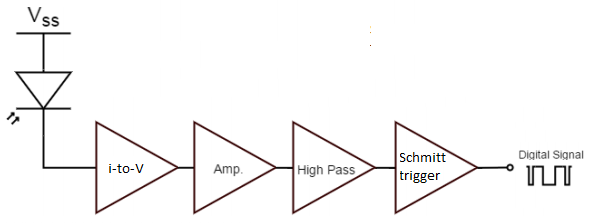
\includegraphics[width=0.8\textwidth]{rec}
\caption{The receiver}
\label{fig:rec}
\end{figure}


\newpage

\subsubsection{Test and simulation results}
The system has proven capable of transmitting asynchronous data with a baud rate of 4800 within a range of 2 meters on land. If a rectangular cointaner filled with water were put in between the transmitter and receiver the range decreasesed to 1 meter. \\\\
The transmission only succeeded if data were sent continuously. If a short break would occur in the continues data stream it takes approximately 20 bytes before the receiver starts outputing valid data again.

\begin{figure}[h]
\centering
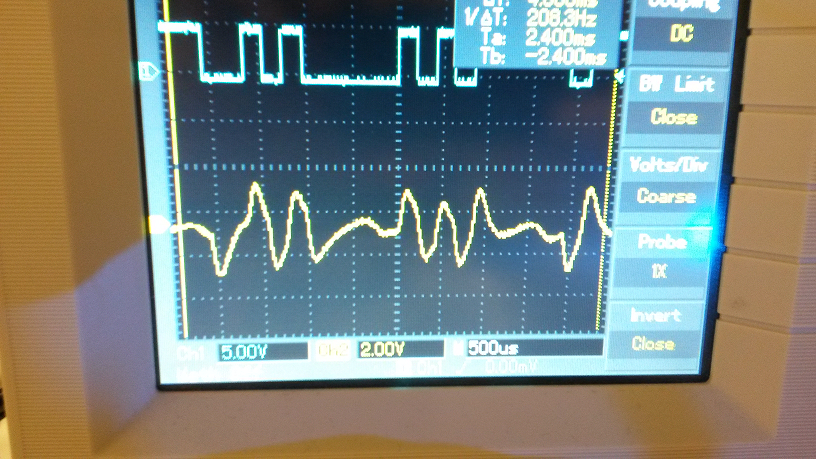
\includegraphics[width=0.8\textwidth]{pic1}
\caption{Filter paramter variation 1  and reconstructed signal}
\label{fig:rec}
\end{figure}

\begin{figure}[h]
\centering
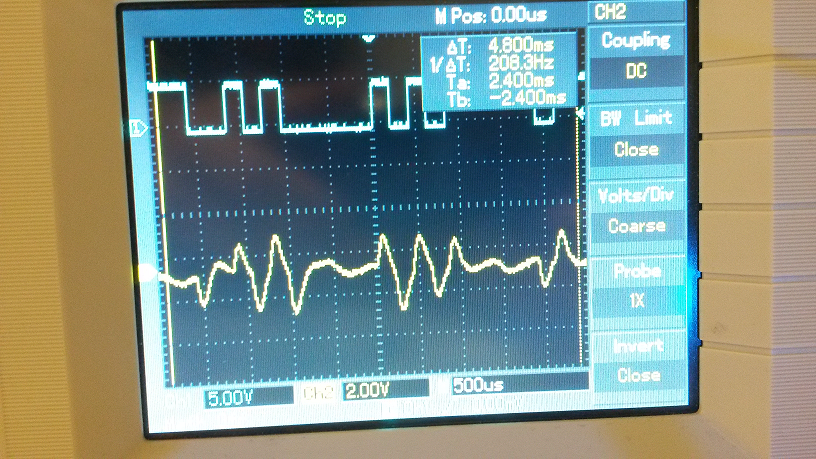
\includegraphics[width=0.8\textwidth]{pic2}
\caption{Filter paramter variation 2 and reconstructed signal}
\label{fig:rec}
\end{figure}




\subsection{Communication part (Sudhangathan Bankarusamy)}

\subsubsection{The prototype}
This setup consists of an LED and photodiode, each of them connected to a Beagle Bone Black(BBB). The LED and photodiode electronic circuits are explained in the electronics section. Figure~\ref{fig:vlc_proto} shows the actual setup. In this prototype version the OpenVLC framework is not used for the lack of time. Instead a simplex serial communication is emulated using light over air.
\begin{figure}
\centering
        \includegraphics[totalheight=8cm]{prototype_VLC.eps}
    \caption{Prototype: Picture of the lab setup}
    \label{fig:vlc_proto}
\end{figure}



\subsubsection{Transmission and receiving of information}
The bits of information is sent to the LED over the serial port, TX, of the BBB. While on the receiving side a photodiode is connected to the RX of the BBB. Any application that uses serial port to transmit information can be used with such a setup. In this case, minicom was used to send and receive characters. Both the BBBs were connected to a laptop. Two different serial terminals were used to connect to both the BBBs and the character send/receive experiment is done. \\
Table~\ref{tab:setupinfo} shows the setup parameters.
\begin{table}[h]
\centering
\caption{Prototype parameters}
\label{tab:setupinfo}
\begin{tabular}{|c|c|}
\hline \textbf{Parameter} & \textbf{Value} \\ 
\hline Baud rate achieved(stable) & 2400 bps \\ 
\hline Distance (stable) & 1.6 m \\
\hline LED power & 1 W \\ 
\hline Wave length & 473nm(Blue) \\ 
\hline Rx pin number(RX BBB) & P9:23 (UART1\_RXD) \\ 
\hline Tx pin number(TX BBB) & P9:24 (UART1\_TXD) \\ 
\hline 
\end{tabular} 
\end{table}



\subsection{Conclusion(Albin Barklund)}
The method works and the technology could probably be used for under water communication even tough it is most likely not a good solution. This is due to the fact arbitrary digital signals contain many different frequencies and the modulation scheme suggests sending all of them through the medium.

\subsection{Future work}
A better approach would be to implement a data link with LEDs and photodiodes which uses a FSK modulation scheme instead.

















